\let\negmedspace\undefined
\let\negthickspace\undefined
\documentclass[journal,12pt,onecolumn]{IEEEtran}
\usepackage{cite}
\usepackage{amsmath,amssymb,amsfonts,amsthm}
\usepackage{algorithmic}
\usepackage{graphicx}
\usepackage{textcomp}
\usepackage{xcolor}
\usepackage{txfonts}
\usepackage{listings}
\usepackage{enumitem}
\usepackage{mathtools}
\usepackage{gensymb}
\usepackage{comment}
\usepackage{caption}
\usepackage[breaklinks=true]{hyperref}
\usepackage{tkz-euclide} 
\usepackage{listings}
\usepackage{gvv}                                        
%\def\inputGnumericTable{}                                 
\usepackage[latin1]{inputenc}     
\usepackage{xparse}
\usepackage{color}                                            
\usepackage{array}                                            
\usepackage{longtable}                                       
\usepackage{calc}                                             
\usepackage{multirow}
\usepackage{multicol}
\usepackage{hhline}                                           
\usepackage{ifthen}                                           
\usepackage{lscape}
\usepackage{tabularx}
\usepackage{array}
\usepackage{float}
%\newtheorem{theorem}{Theorem}[section]
%\newtheorem{theorem}{Theorem}[section]
%\newtheorem{problem}{Problem}
%\newtheorem{proposition}{Proposition}[section]
%\newtheorem{lemma}{Lemma}[section]
%\newtheorem{corollary}[theorem]{Corollary}
%\newtheorem{example}{Example}[section]
%\newtheorem{definition}[problem]{Definition}

\begin{document}

\title{2.2.28}
\author{AI25BTECH11035 - SUJAL RAJANI}
% \maketitle
% \newpage
% \bigskip
%\begin{document}
{\let\newpage\relax\maketitle}
%\renewcommand{\thefigure}{\theenumi}
%\renewcommand{\thetable}{\theenumi}
% \newpage
% \bigskip
\textbf{Question}:
\\
 Find the angle between the two planes 2x+y-2z=5 and 3x-6y-2z=7 using vector method.
 \\
 \textbf{Solution}
 \\
 the   normal vector of plane 2 x+y-2z=5 is : $\vec{A}$
 \begin{align*}
     \vec{A}=\myvec{2\\1\\-2}
 \end{align*}
 the normal vector of plane 3 x-6y-2z=7 is : $\vec{B}$
 \begin{align*}
     \vec{B}=\myvec{3\\-6\\-2}
 \end{align*} 
 The value of $||\vec{A}||$:
  \begin{align*}
     (\vec{A})^T(\vec{A})={||\vec{A}||}^2=9
 \end{align*}
 The value of $||\vec{B}||$:
  \begin{align*}
     (\vec{B })^T(\vec{B})={||\vec{B}||}^2=49
 \end{align*}
 The angle between two plane is same as the angle between their normal vectors , which is  $\theta$ .
\\
\\
 the angle between $\vec{A}$ and $\vec{B}$ is :
 \begin{align*}
      \cos{\theta} = \dfrac{(\vec{A})^T(\vec{B})}{||\vec{A}||\quad||\vec{B}||}=\dfrac{4}{21}
      \\
      \theta=cos^{-1}\dfrac{4}{21}
 \end{align*}
        \begin{figure}[H]
    \centering
    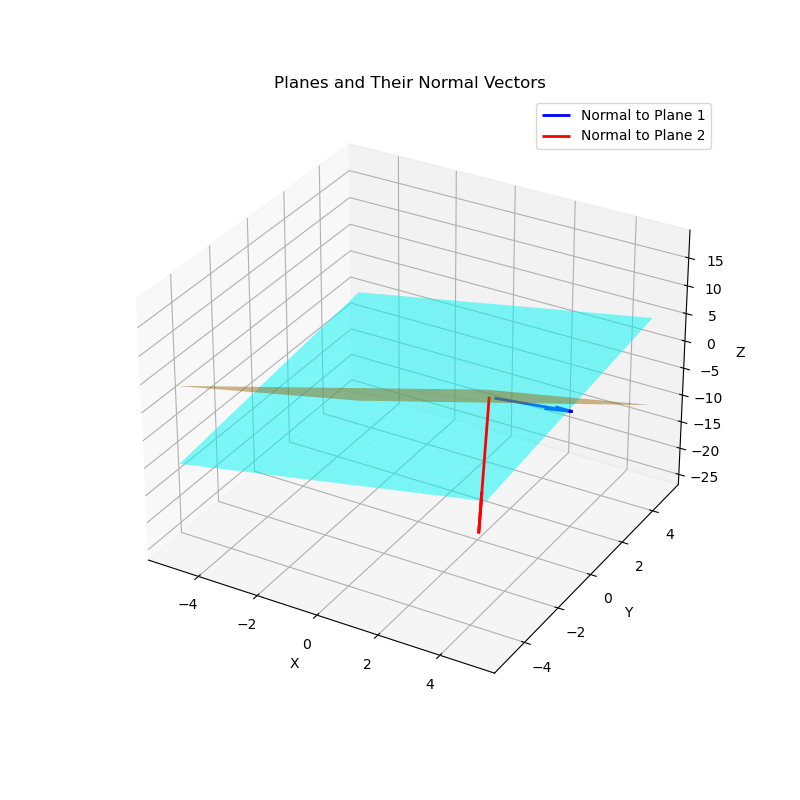
\includegraphics[width = 0.7\columnwidth]{figs/img.png}
    \caption*{}
    \label{figs}
\end{figure}

\end{document}